% WSCG sample document 
%
% based on Gabriel Zachmann's sample
% http://zach.in.tu-clausthal.de/latex/
%
% modified Apr 2012 to match WSCG Word template
%
\documentclass[twoside,twocolumn,10pt]{article}



%%%%%%%%%%%%%%%%%%%%%%%%%%%%%%%%%%%%%%%%%%%%%%%%%%%%%%%%%%%%%%%%%%%%%%%%%%%%%
%                             Packages

\usepackage{wscg}           % includes a number of other packages (e.g., myalgorithm)
\RequirePackage{ifpdf}
\ifpdf
 \RequirePackage[pdftex]{graphicx}
 \RequirePackage[pdftex]{color}
\else
 \RequirePackage[dvips,draft]{graphicx}
 \RequirePackage[dvips]{color}
\fi


\usepackage{nopageno}       % no page numbers at all; uncomment for final version

\usepackage{subfig}
\usepackage{graphicx}
\usepackage[justification=centering]{caption}
\usepackage{amsmath}
\usepackage[linesnumbered,ruled]{algorithm2e}
\usepackage[english]{babel}
%%%%%%%%%%%%%%%%%%%%%%%%%%%%%%%%%%%%%%%%%%%%%%%%%%%%%%%%%%%%%%%%%%%%%%%%%%%%%
%                                Title

\title{MAELab: a framework to automatize landmarks setting}

\author{
  \hspace{-0.1\textwidth}
  \parbox{0.2\textwidth}{\centering
    LE Van \\
    Linh\\[1mm]
LaBRI-CNRS 5800\\
ITDLU, Dalat Univ-V
linhlv@dlu.edu.vn/ van-linh.le@labri.fr
}
\hspace{0.02\textwidth}
\parbox{0.2\textwidth}{\centering
BEURTON-AIMAR Marie\\[1mm]
LaBRI-CNRS 5800\\
Bordeaux University\\
33400 Talence-F\\
beurton@labri.fr
}
\hspace{0.02\textwidth}
\parbox{0.25\textwidth}{\centering
KRAHENBUHL \\Adrien\\[1mm]
LaBRI-CNRS 5800\\
Bordeaux University\\
33400 Talence-F\\
adrien.krahenbuhl@labri.fr
}
\hspace{0.02\textwidth}
\parbox{0.18\textwidth}{\centering
PARISEY\\ Nicolas\\[1mm]
IGEPP\\
INRA 1349\\
35653 Le Rheu-F\\
nparisey@rennes.inra.fr
}
}

%%%%%%%%%%%%%%%%%%%%%%%%%%%%%%%%%%%%%%%%%%%%%%%%%%%%%%%%%%%%%%%%%%%%%%%%%%%%%
%                          Hyperref


% no hyperlinks
\usepackage{url}
\urlstyle{tt}

% Donald Arsenau's fix for missing kerning of "//" and ":/"
\makeatletter
\def\Uslash{\mathbin{\mathchar`\/}\@ifnextchar{/}{\kern-.15em}{}}
\g@addto@macro\UrlSpecials{\do \/ {\Uslash}}
\def\Ucolon{\mathbin{\mathchar`:}\@ifnextchar{/}{\kern-.1em}{}}
\g@addto@macro\UrlSpecials{\do : {\Ucolon}}
\makeatother




%%%%%%%%%%%%%%%%%%%%%%%%%%%%%%%%%%%%%%%%%%%%%%%%%%%%%%%%%%%%%%%%%%%%%%%%%%%%%
%                                Document


\begin{document}

\twocolumn[{\csname @twocolumnfalse\endcsname

\maketitle  % full width title


\begin{abstract}
\noindent  Phenotype of insect species are characterized by several informations like
  age, sex, morphological measures or environmental parameters. Biologists are
  familiar to manually get morphological measures and in the case of
  analysis at the macro level (tissues, small parts of the animal \ldots)
  they can do directly by measuring the element geometry: length,
  width, diameter, angles, \ldots. Another way to obtain morphological
  measures is to take pictures of
  these elements and to run image processing algorithms. In order to
  evaluate a population of beetles into Brittany lands, a collection of
  293 beetles has been built. For each beetle, the images of the left
  and right mandibles are available and a set of 16 and 18
  landmarks (resp. left and right) have been manually set, given 
  the ground truth to compare to the estimated landmarks. In a previous
  work \cite{leestimating} based on Palaniswamy article \cite{palaniswamy2010automatic}, we have shown that the probabilistic Hough Transform (PHT) can provide very
  interesting results if we consider the centroid measure of the mandible as the parameter
  to obtain. But if the goal is to consider more precisely
  the position or the geometry of landmark areas, the results are not
   accurate enough to consider the estimated landmarks instead of manual landmarks. In this
   paper, we have improved the previous algorithms
   of segmentation based on Canny algorithm, and we have preferred a registration
   procedure based on an iteration of the Principal Component Analysis
   calculus. To achieve the estimated landmarks setting we have
   computed a SIFT descriptor limited to the landmarks area in the
   model and correlated it to the scene image. A workflow, MAELab, has been
   written, containing all the operations; it is freely available as library functions on a GitHub website.
\end{abstract}

\subsection*{Keywords}
Automatic morphology, landmarks identification, image registration.

\vspace*{1.0\baselineskip}
}]



%%%%%%%%%%%%%%%%%%%%%%%%%%%%%%%%%%%%%%%%%%%%%%%%%%%%%%%%%%%%%%%%%%%%%%%%%%%%%


\section{Introduction}

\copyrightspace
In biology, morphology analysis is widely used to keep the changing
information of the organism or detecting the difference information
between the organisms. From the result of morphology analysis, we can
determine the evolution of an organism family, or we may classify the
organisms. Especially in agriculture, morphology is one of best ways
to learn about the variations of the insect on crops. The morphology
methods may be divided into groups by features which are used
by the methods. The features can be such as shape, structure, color, pattern or size of the
object. In the aim to study the potential links between these
variations and agricultural ecosystems, a set of beetles has been
collected with all informations about the sex, place where they were
found and agricultural practices in each field were recorded. For each
beetle, morphometric landmarks has been manually set on the images of
the left and right mandibles. The morphometric landmarks are points precisely defined by biologists. Landmarks are
widely used in many biological studies and they are currently included
into the classification procedures.\\[0.1cm]


\begin{figure}[h]
\centering
\subfloat[Left mandible]{\label{figrbox2}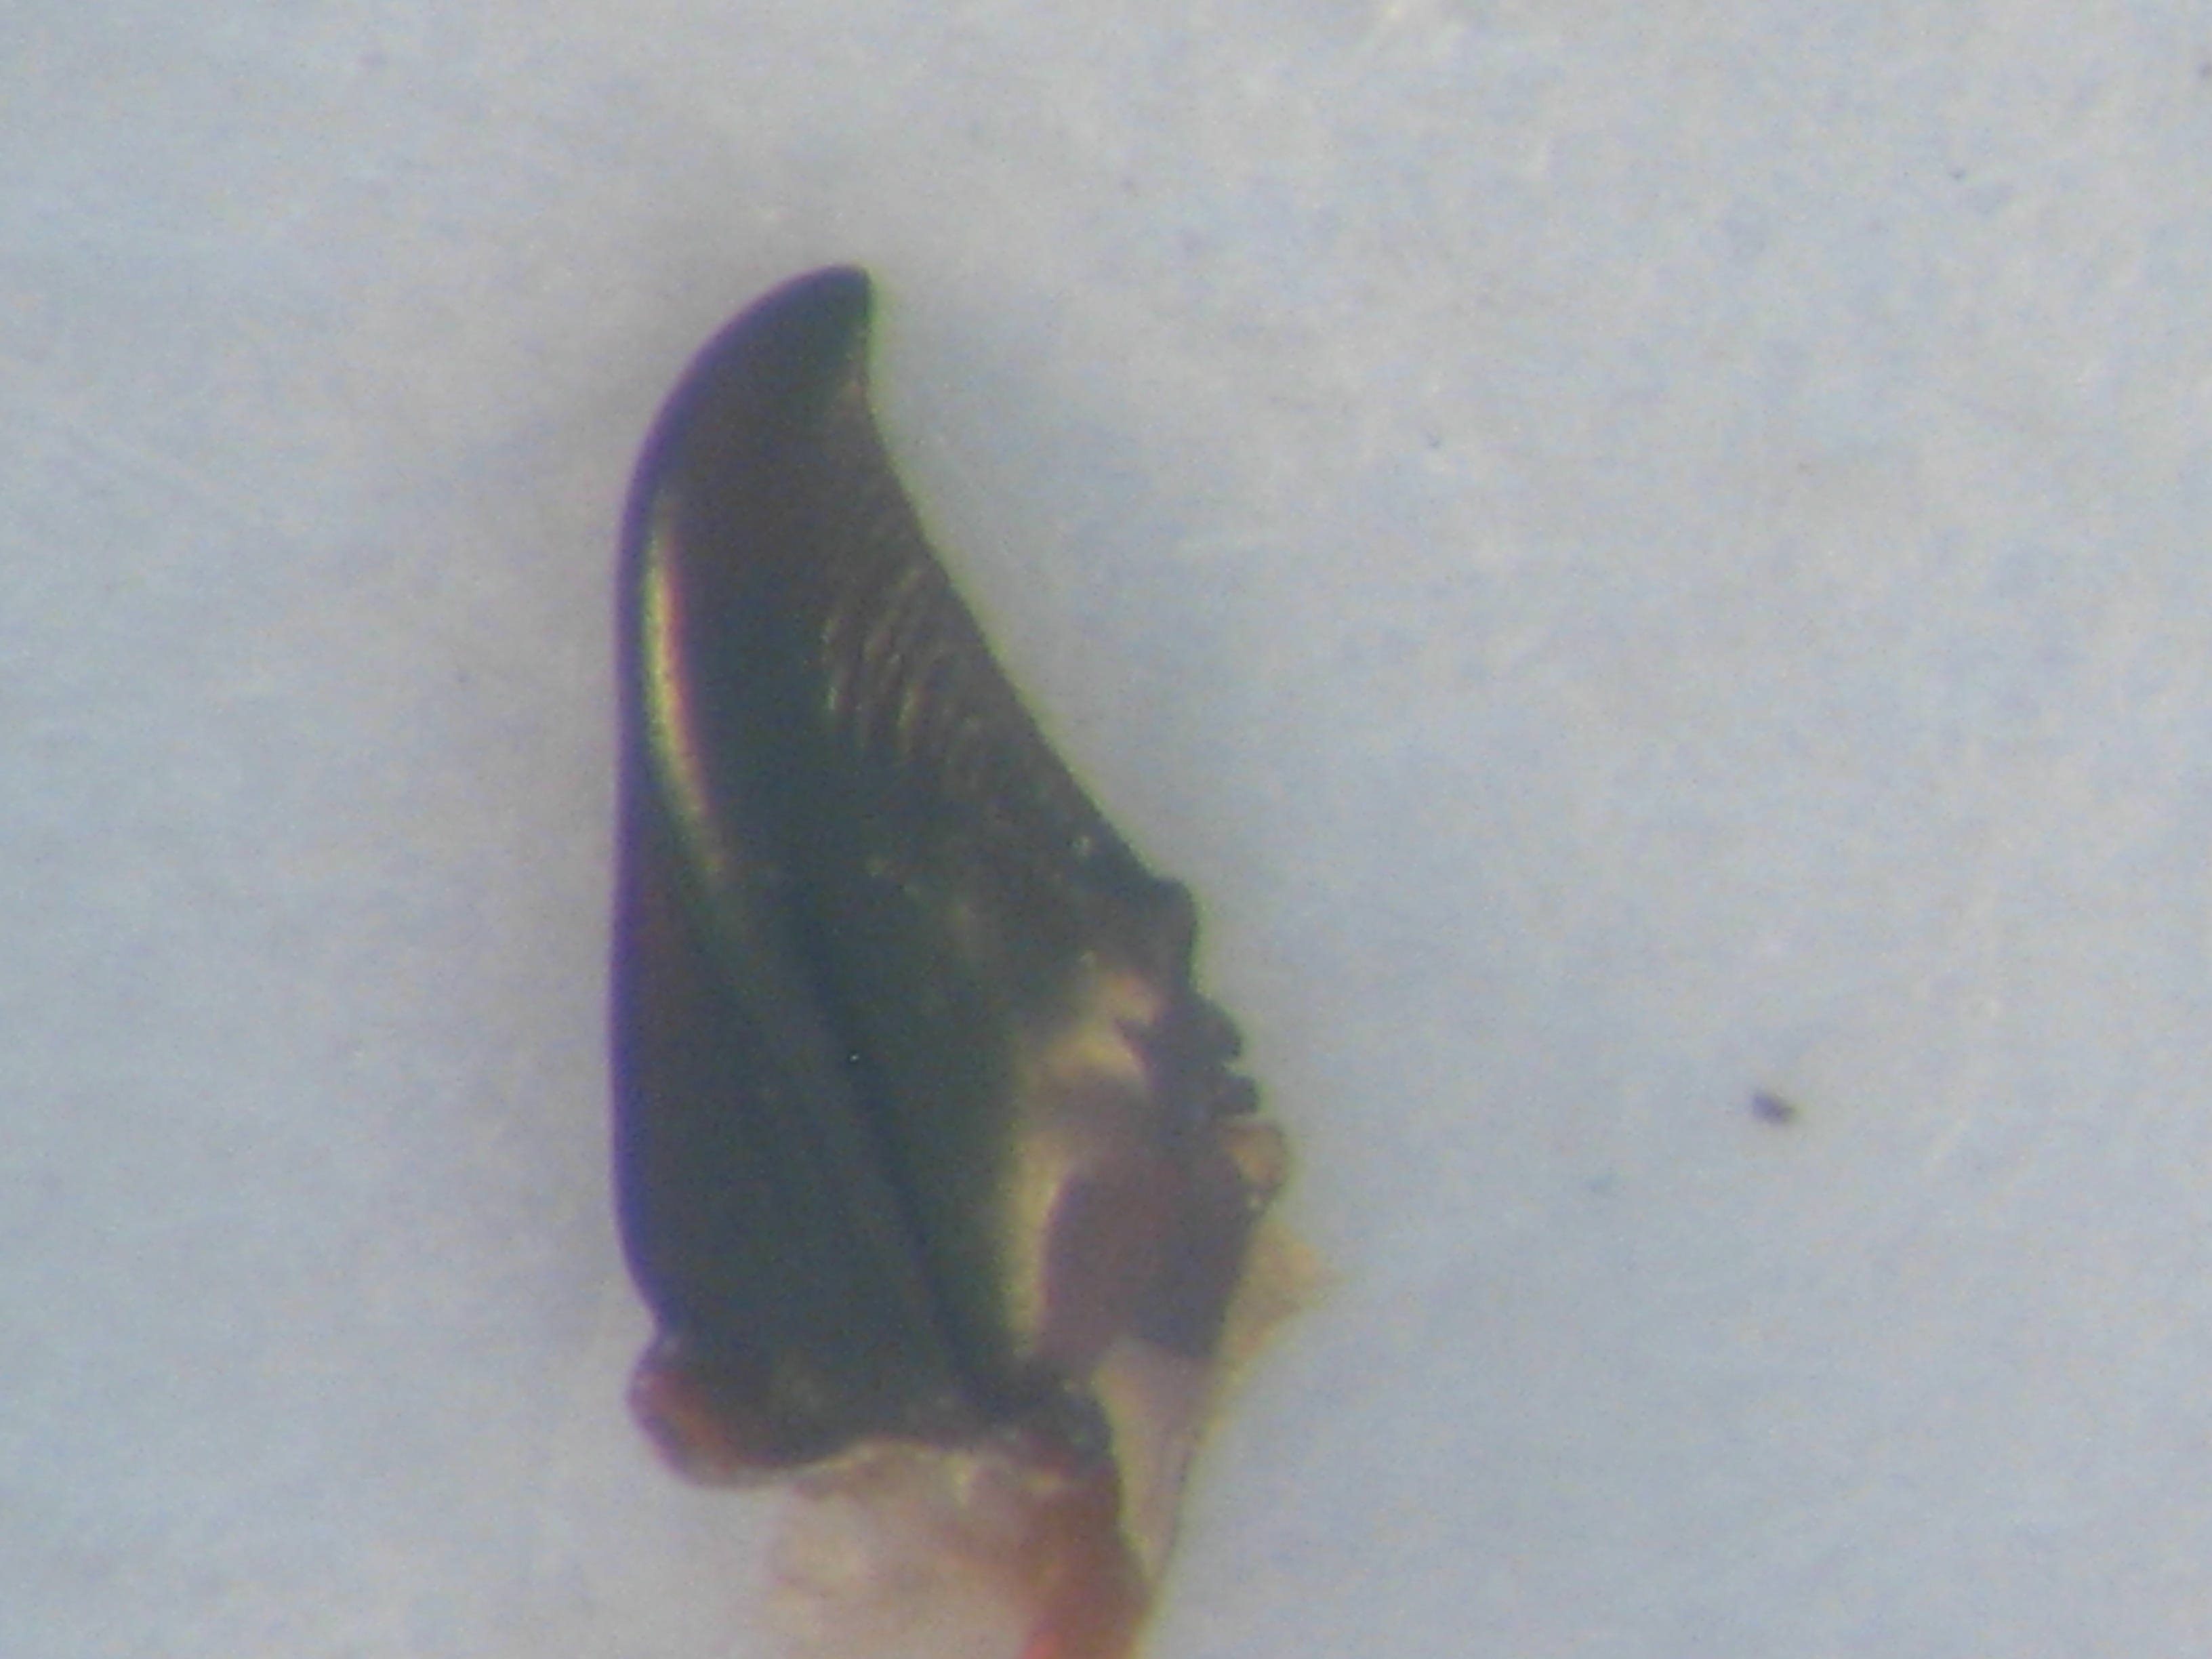
\includegraphics[width=0.22\textwidth]{./images/lm}}~~
\subfloat[Right mandible]{\label{figrbox1}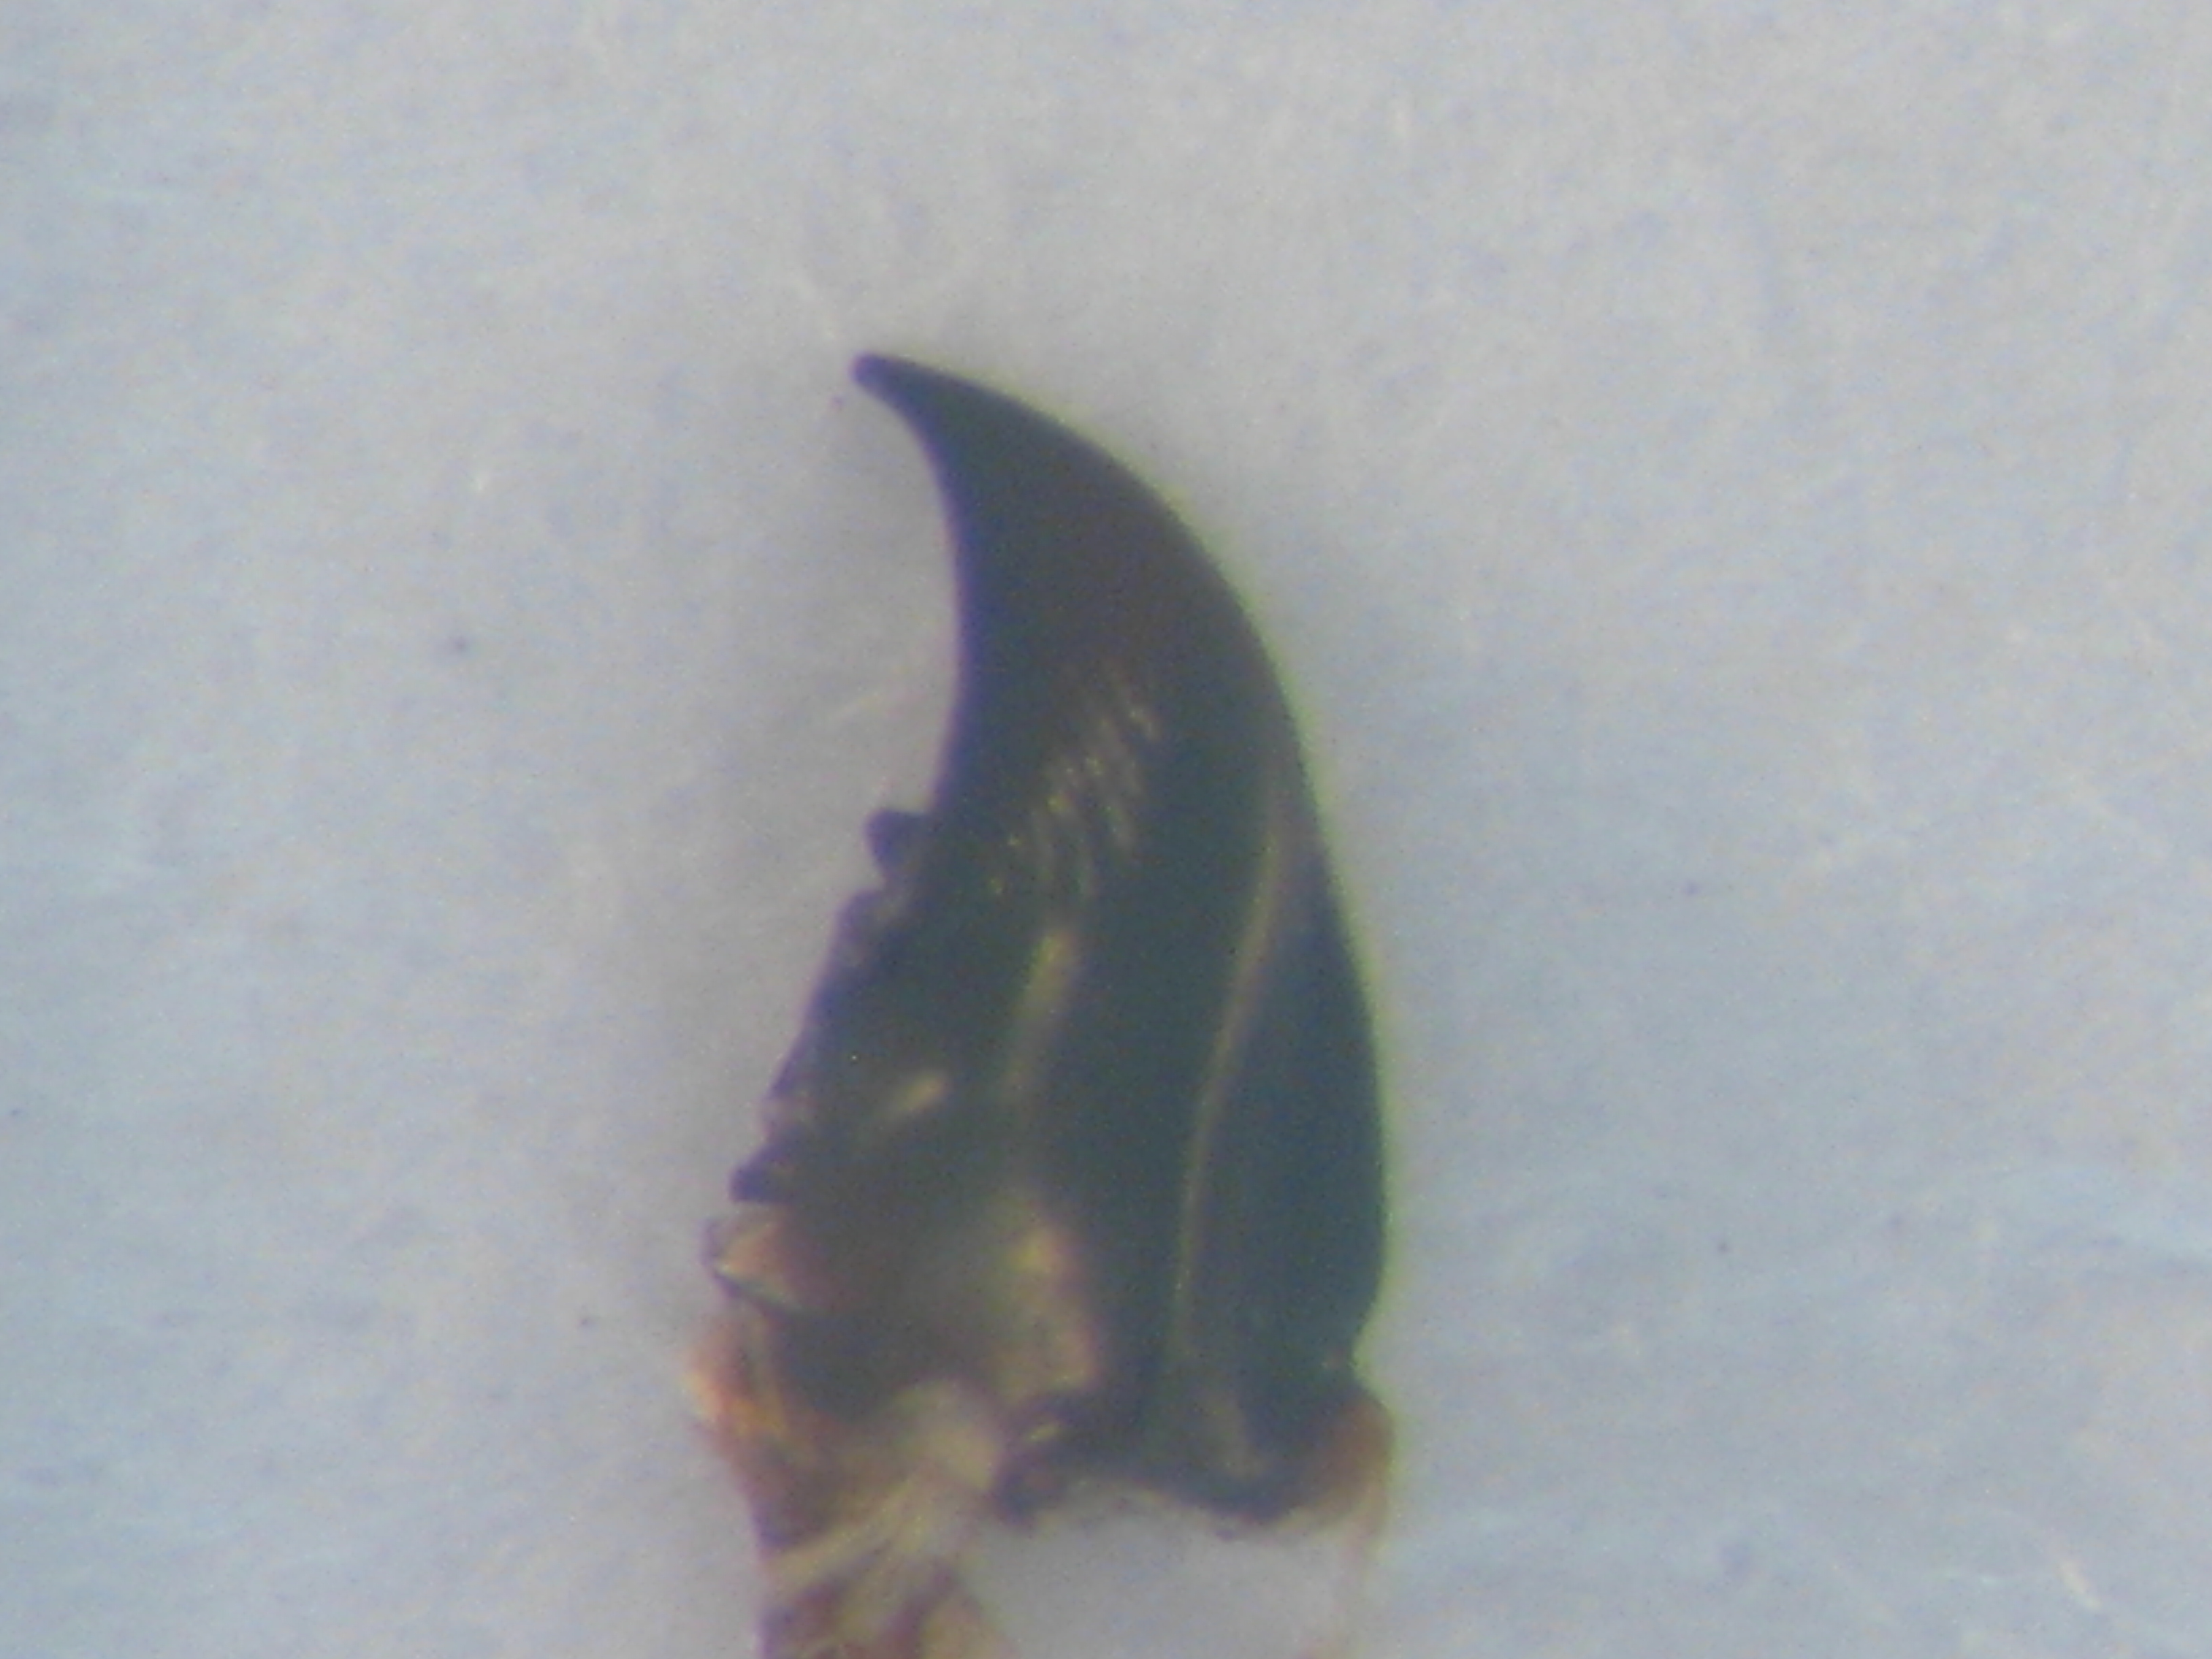
\includegraphics[width=0.22\textwidth]{./images/rm}}
\caption{The mandibles of beetle}
\label{figparts}
\end{figure}~\\[0.1cm]
In this paper, we focus on a chain of algorithms to automatically identify  landmarks on our 2D images. The method
mainly includes three stages: firstly, we segment the shape of the
mandible, then principal component analysis iteration is 
used to register one model image with a scene, the translation and
rotation between the two images are also determined; finally, the
landmarks are estimated by a method using a SIFT descriptor.\\

In section 2, we present the steps of our method. All
experiments and evaluations are then described in section 3. 

\section{Method}
The problem to solve is to suppress the manual operation of setting
landmarks on each image. To do that, we propose a workflow, including the segmentation of each image and a registration
with a model image. The model image is chosen randomly from the images without broken mandibles. The figure \ref{fig:method} shows the steps of the workflow: \\
%%we need to change the drawing a little bit
\begin{figure}[htb]
    \centering
    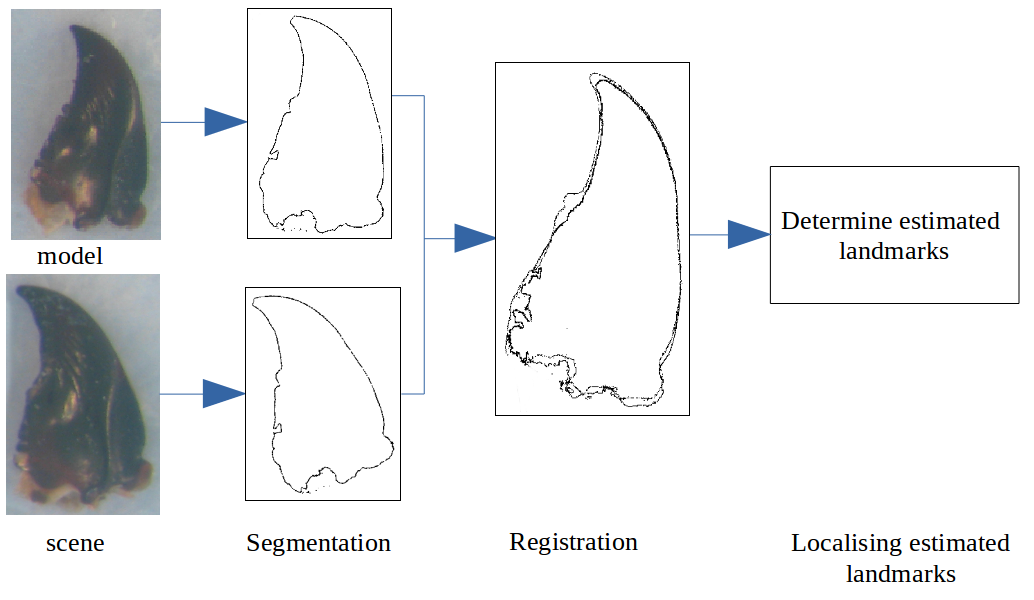
\includegraphics[width=0.5\textwidth]{./images/method}
    \caption{Overview of the proposed method}
    \label{fig:method}
\end{figure}~\\
In this section, we will describe the different algorithms that we have
used. It is worth to note that all pictures of mandibles have
been taken in the same conditions with the same camera at the same resolution.
\subsection{Image segmentation}
Segmentation is often the first major task of an image processing
chain. The most well-known algorithms are classified as contour
or region based approaches. We have chosen a contours one, the
Canny alogrithm \cite{canny1986computational}, allowing to determine the 
list of edges belonging to the shape of the image.
To use this method, two threshold values have to be set. As it is often mentioned, determine the right values for these thresholds could be difficult\cite{adaptiveCanny}. The mandatory \textit{threshold
  value} used by Canny algorithm has been determined by analyzing the image
histogram (see \cite{leestimating} for detail). Most often authors define from this threshold, a lower and an upper one. The usual ratio of these two thresholds is $T_{lower} = (1/2) * T_{upper}$. In order to consider a larger range of values, we have prefer to set $T_{lower}$ to $1/3$ of $T_{upper}$. For optimization the computing time, the gradient direction of each pixel which belongs to the contours is computed during the Canny algorithm to be used later.\\
\begin{figure}[h]
\centering
\subfloat[Segmentation result after applying Canny
  algorithm]{\label{canny1}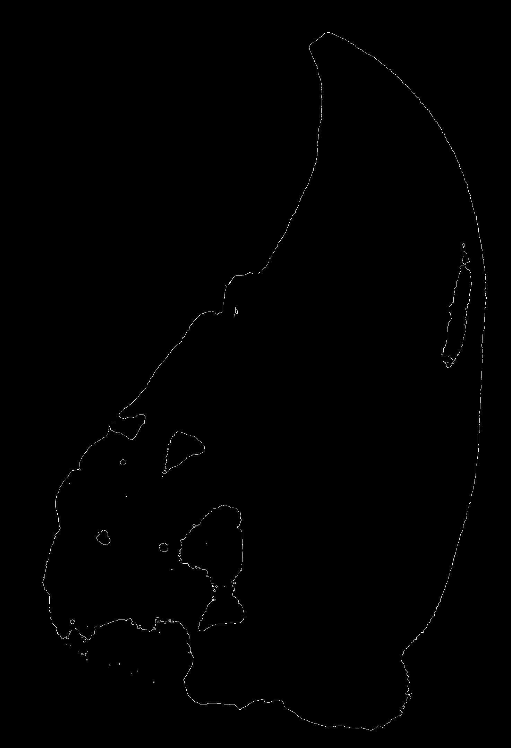
\includegraphics[width=0.2\textwidth]{./images/canny1}}~~ 
\subfloat[Segmentation result after applying Canny algorithm and
  post-process]{\label{canny2}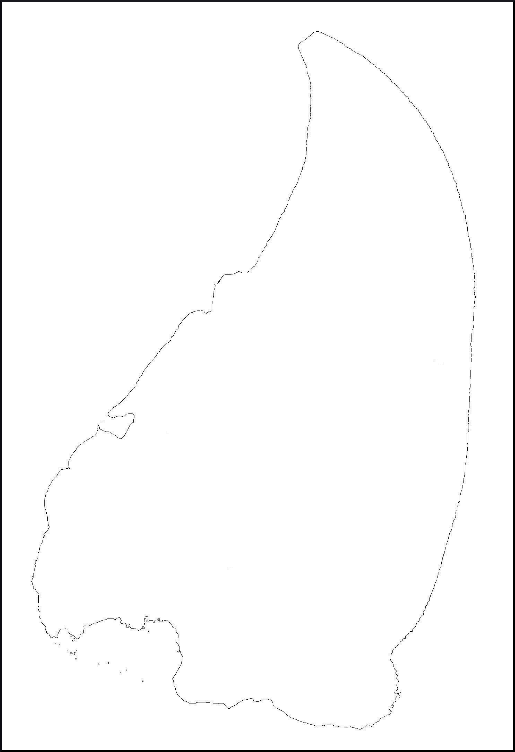
\includegraphics[width=0.2\textwidth]{./images/canny2}} 
\caption{The segmentation results of the image}
\label{canny}
\end{figure}~\\
To achieve the segmentation, the obtained contours are post-processed to remove unnecessary
ones. As it is shown in figure \ref{canny}, the final result of Canny generates some contours which do not belong to the shape of the mandible. With a simple algorithm, we browse the image and suppress the edges inside the main shape.
\subsection{Image registration}
As mentioned, all images have been captured following the same protocol at the same scale. But it remains differences in size between the mandibles cause of size of the beetles, or orientation and position because of the mandible position under the camera. The next step concerns registration of model and scene before estimating the landmarks. Principal Component Analysis (PCA) is a well-known method to find the rotation and translation parameter values between two images. In our workflow, we have first used a classical PCA computing \cite{bsspca}, \cite{shlens2014tutorial}.\\
As input values, we use the lists of points which have been defined by the segmentation step. Firstly, the centroid point and principal axis of each image are defined: the centroid point is the point which has the coordinate equal to the mean coordinate of all boundary points; the principal axis is a connected line from the centroid point to a point in the list of contours points which is determined as detailed in algorithm \ref{alg1}:
\begin{algorithm}
	\SetKwInOut{Input}{Input}
	\SetKwInOut{Output}{Output}
	\Input{Centroid point, list points of contours}
	\Output{The principal axis}
	\For{ all points $i$ in the list of contour points}
	{
		Draw line $l$ between $i$ and $centroid$ point;\\
		\For{ all points $j$ in the list of contour points}
		{
			\If{$i \neq j$}
			{
				Compute the perpendicular distance $P_d$ between line $l$ and point $j$;\\
			}		
		}
		Compute the average ($P_{mi}$) of all $P_d$;\\
		\If{$P_{mi}$ is minimal}
		{
			Store $i$ as $i_{min}$;\\
		}
	}
	The principal axis is the line between $centroid$ and $i_{min}$.
	\caption{The algorithm for finding the principal axis of a list of contour points}
	\label{alg1}
\end{algorithm}\\

The translation is calculated by the distance of the centroid point of the scene and the model. The rotation angle is the angle between the principal axes of these two images. Then, the scene is moved to be register with the model. However,
in some cases, the translation and rotation between two images are
not enough precise because the result of the segmentation could be not perfect. To improve registration, we have enhanced the PCA by iteration steps (PCAI). We have considered some specificity of our images and observed that the tip of mandible is less noisy than the base. So, we sort the points according to their y-value. We build a subset of points which contains half part of points, these ones belonging to the upper part of the image. PCA is again completed for this subset to refine the rotation and translation values. This operation is iterated until the new computing angle is less than 1.5 degree (see figure \ref{fig:pcai}).
\begin{figure}[htb]
    \centering
    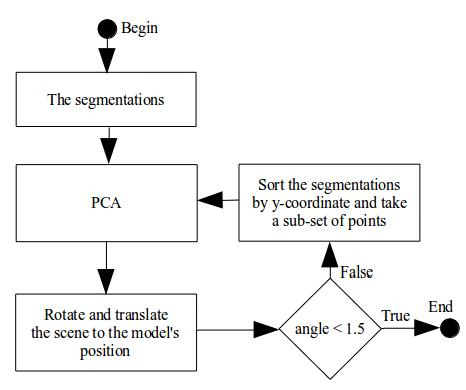
\includegraphics[width=0.45\textwidth]{./images/pcadiagram}
    \caption{The flows in PCAI}
    \label{fig:pcai}
\end{figure}~\\
Figure \ref{fig:box} shows an example of obtained results from the different steps of PCAI. In this figure, the red contours is the model segmentation, the black contours is the scene segmentation after one iteration, and the blue contours is the last result of PCAI .\\

\begin{figure}[htb]
    \centering
    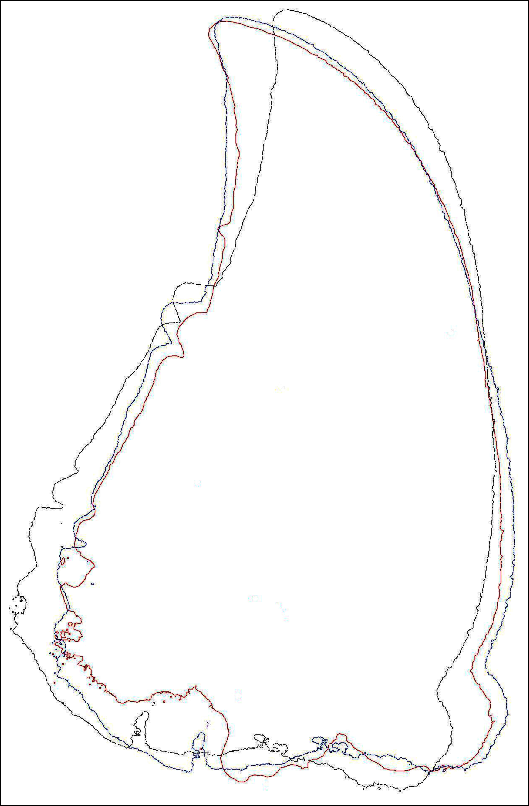
\includegraphics[width=0.3\textwidth]{./images/imreg}
    \caption{Different registration steps between two images}
    \label{fig:box}
\end{figure}
\subsection{Localising the estimated landmarks}
The last task of the workflow consists to estimate the landmarks of the scene from the manual ones of the model. We use SIFT \cite{lowe2004distinctive} method. But we do not consider all points of the image as usually, only the area around the landmarks. Firstly, the region around each manual landmark (called patch) in the model is extracted and its corresponding position in the scene image is defined. Then, the SIFT descriptor is computed: the orientation and gradient magnitude are calculated for each pixel by using the gradient values computed at the Canny step and applying the equations (\ref{eq:sift}):
%\begin{equation}
%\label{eq:sift}
%\resizebox{.5 \textwidth}{!} 
%{$
%\begin{aligned}
%	m(x,y) = \sqrt{(P(x+1,y) - P(x-1,y))^2 + (P(x,y+1) - P(x,y-1))^2} \\
%	\theta(x,y) = tan^{-1}((P(x,y+1) - P(x,y-1))/(P(x+1,y) - P(x-1,y)))
%	\end{aligned}
%$}
%\end{equation}
\begin{equation}
\label{eq:sift}
\begin{split}
	m(x,y) &= \sqrt{P_x^2 + P_y^2} \\
	\theta(x,y)& = tan^{-1}(P_y/P_x) \\
	(P_x &= P(x+1,y) - P(x-1,y) \text{ and } \\
	P_y &= P(x,y+1) - P(x,y-1) )
\end{split}
\end{equation}
Where:
\begin{itemize}
	\item $P(x,y)$ is the gray value at position (x,y) in the patch,
	\item $m(x,y)$ is the gradient magnitude of the pixel at position (x,y),
	\item $\theta(x,y)$ is the orientation of the pixel at position (x,y).
\end{itemize}
The SIFT descriptor for each patch is an histogram which contains the sum of pixels gradient for each considering direction. As usually, eight directions are take into account ($0^o - 45^o$, $46^o - 90^o$, $91^o - 135^o$, $136^o - 180^o$, $181^o - 225^o$, $226^o - 270^o$, $271^o - 315^o$, $316^o - 360^o$). Finally, the feature vector is normalized to reduce the effects of illumination changes.

\begin{figure}[htb]
    \centering
    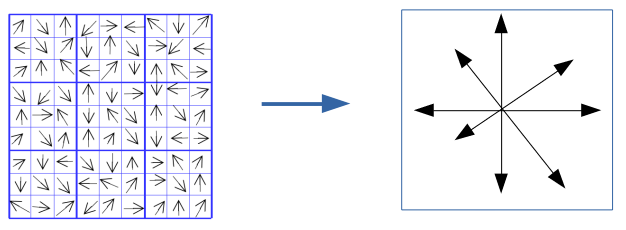
\includegraphics[width=0.4\textwidth]{./images/keypoint_descriptor}
    \caption{Calculus of the global descriptor for a patch. Gradient value is arrow length in the right figure}
    \label{fig:kpdescriptor}
\end{figure}
The figure \ref{fig:kpdescriptor} shows sample of a patch of 9x9 pixels created around each landmark on the model. The landmark of the model is located in the center of the patch. The size of 9x9 has been retained after several tests. Patch sizes: 18x18, 36x36, 54x54 have been also computed and gave us results statistically worst. From the histogram of the patch, we obtained the global gradient value for each direction.\\

The comparison between two SIFT descriptors is done by using $L2$ distance, equation (\ref{eq:L2distance}).
\begin{equation}
\label{eq:L2distance}
	L(D1,D2) = \sum\limits_{i = 0}^{n}\sqrt{(D1_i-D2_i)^2}
\end{equation}
Where:
\begin{itemize}
	\item $n$ is the number of directions
	\item $D1$ and $D2$ are two descriptors with size $n$,
	\item  $D1_i$, $D2_i $ are the value at the location $i$ in each descriptor.
\end{itemize}
Figure \ref{fig:Illustrate} illustrates how we apply SIFT into our work. To fix model landmarks on the scene, the patches \textit{$P_m$, $P_s$} are created with size($P_m$) $<$ size($P_s$). After experiments, we keep 36 (pixels) as the size of \textit{$P_s$}. For each pixel in the patch \textit{$P_s$}, a sub-patch \textit{$P^{'}_s$} is extracted with the same size than \textit{$P_m$}. When the \textit{$P^{'}_s$} is not possible to get from \textit{$P_s$} (border limits), the pixels outside \textit{$P_s$} are more considered. Then, the distance \textit{$L(P_m,P^{'}_s)$} is computed by (\ref{eq:L2distance}). This process is finished when all the pixels on the patch \textit{$P_s$} are considered. The coordinates of an estimated landmark is the location in \textit{$P_s$} that has the smallest measure distance value with \textit{$P_m$}. Finally, the coordinates of the estimated landmarks are set to the original location of the scene by applying the reverse operation of rotation and translation.
\begin{figure}[htb]
    \centering
    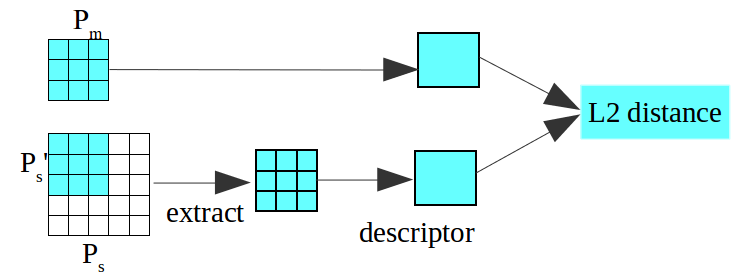
\includegraphics[width=0.48\textwidth]{./images/illustration_SIFT}
    \caption{Illustrate the steps of descriptors comparison.}
    \label{fig:Illustrate}
\end{figure}
\section{Experiments and result}
All the steps of our method are implemented in MAELab\footnote{MAELab
  is a free software in C++. It can be directly obtained by request
  the authors.}. The set of beetles has been analyzed, right and left
mandibles. After verifying the quality of the image, it remains 290
usable images of right mandible and 286 images of the left mandible. The
removed images include the images that do not contain the mandible or
the broken mandibles. In all valid images, a set of manual landmarks are indicated by 
biologists: 18 for right mandibles, 16 for left mandibles.\\

We have run the full workflow on all images. The preliminary results have shown differences in algorithm accuracy: estimated landmarks are well positioned on some scenes but not satisfying on others. As we mentioned before, mandibles can exhibit different sizes because beetles have also. It seems that our method is sensible to this parameter. To improve our results, we have inserted a step before computing SIFT descriptor to estimate the scale between one scene image and the model. The bounding boxes of the mandible of the model image and the scene image are computed and the scales of x and y-direction are determined by the ratio between the corresponding sides of the bounding boxes. Then, the scene contours are scaled to fit the model contours. \\
\begin{figure}[h]
\centering
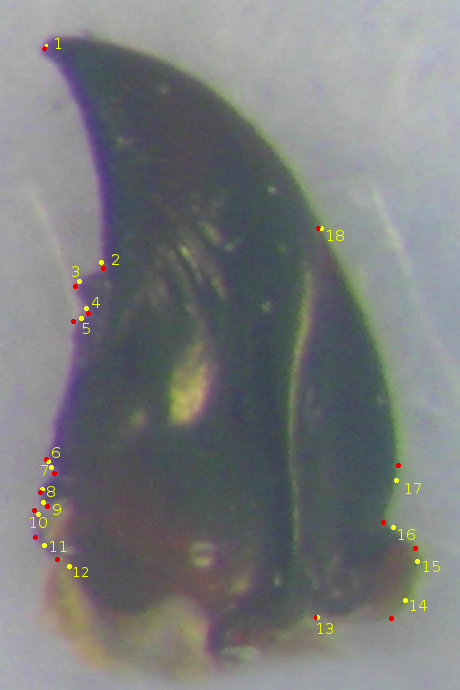
\includegraphics[width=0.35\textwidth]{./images/md_rs}
\caption{The manual and estimated landmarks on right mandible}
\label{figresult}
\end{figure}~\\
\begin{figure}[h]
\centering
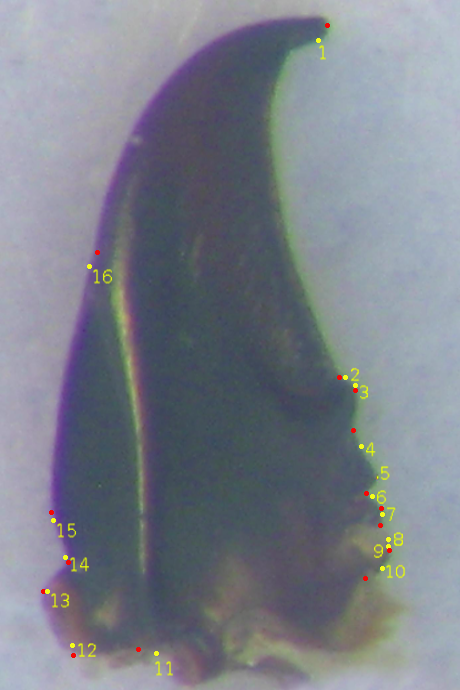
\includegraphics[width=0.35\textwidth]{./images/mg_rs}
\caption{The manual and estimated landmarks on left mandible}
\label{figresult2}
\end{figure}~\\

Figure \ref{figresult} and \ref{figresult2} show complete results on one right mandible and one left mandible with the manual landmarks (red points) and estimated landmarks (yellow points). The estimated landmarks are quite near with the manual landmarks. This shows that our method works well for indicating the landmarks on the mandibles.\\

In the evaluation, the statistic is done on all landmarks of the images. We have compared the coordinates between the manual and estimated landmarks and accept the error in the range between 1\% to 2\% of the bounding box's size. According to this way, a global statistic compares all pairs of landmarks (manual and corresponding estimated landmarks) on all images.
\begin{figure}[h]
\centering
\subfloat[Right mandibles]{\label{figmdresult}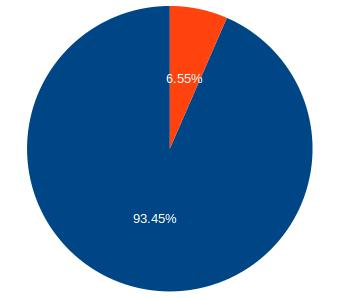
\includegraphics[width=0.22\textwidth]{./images/mdresult}}~~
\subfloat[Left mandibles]{\label{figmgresult}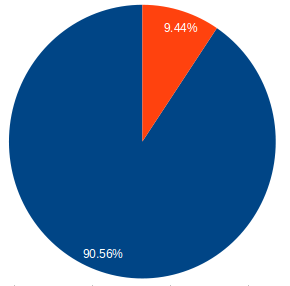
\includegraphics[width=0.22\textwidth]{./images/mgresult}}
\caption{The global proportions of well and bad landmark locations on the mandibles}
\label{figctresult}
\end{figure}~\\
Figure \ref{figctresult} shows the global results: we have obtained \textbf{87.03}\% for right mandibles and \textbf{78.82}\% for left mandibles of well positioned estimated landmarks.\\

Besides the global results, we are also
interested in the accuracy of the individual position of the estimated landmarks. We have computed the distance between the manual and corresponding estimated landmarks in order to examine the correct proportion on each landmark and think about replacing the manual landmarks by corresponding estimated landmarks.
\begin{figure}[htb]
    \centering
    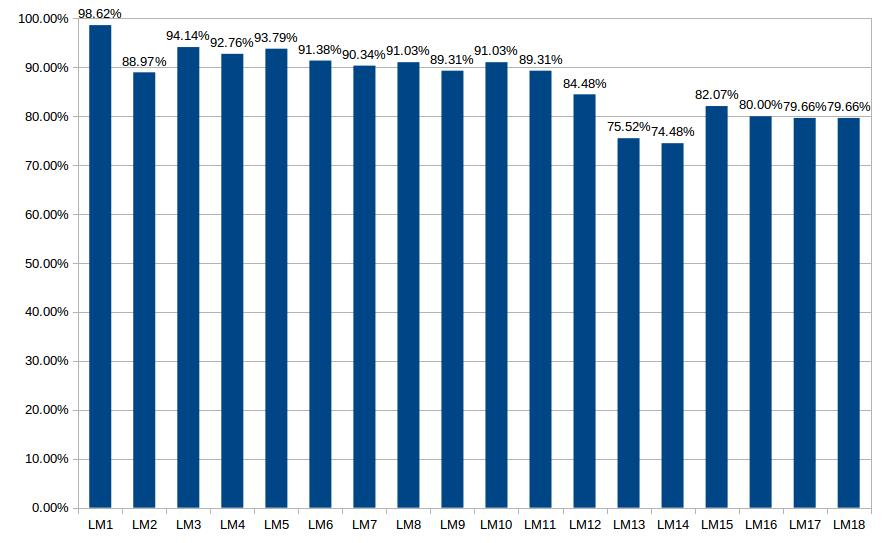
\includegraphics[width=0.5\textwidth]{./images/md_chartlms}
    \caption{The correct proportions on each landmark of right mandibles }
    \label{figmdresultlm}
\end{figure}~\\
\begin{figure}[htb]
    \centering
    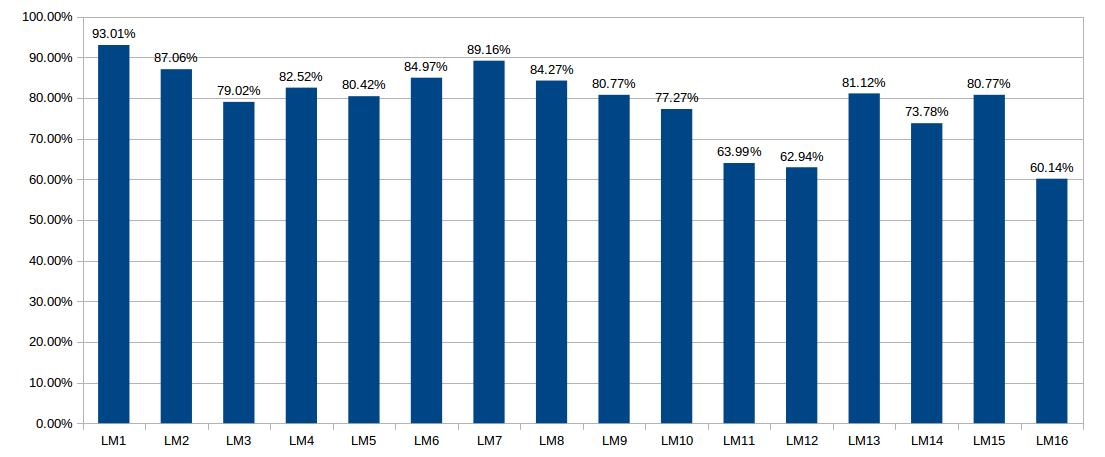
\includegraphics[width=0.5\textwidth]{./images/mg_chartlms}
    \caption{The correct proportions on each landmark of left mandibles }
    \label{figmgresultlm}
\end{figure}~\\
Figure \ref{figmdresultlm} and \ref{figmgresultlm} show the correct proportion on each landmark of the mandibles. With 18 landmarks of right mandible, the position of the first estimated landmarks is reasonably accurate with \textbf{98.62}\%, the lowest proportion is \textbf{74,48}\% for fourteenth landmark. The remaining landmarks are also indicated with a high proportion (with the accuracy proportion greater than 75\%). For left mandible, the highest and lowest success rate are \textbf{93,01}\% for the first landmark and \textbf{60,14}\% for the sixteenth landmark. The statistic is done on each estimated landmarks of all the images with a standard deviation error \cite{bland1996statistics}. As we can see in figure \ref{canny}, the noise of the contour part located at the base of mandible is higher than the noise located at the tip of the mandible. This explains why the correct proportion on $11^{th}$, $12^{th}$ landmark of the left mandible or $13^{th}$, $14^{th}$ landmark of the right mandible are less than other landmarks. Moreover, when we reconsider the datasets, the images in left mandible have a higher number of scales than on the right mandible. This explains the success rate on the right mandible is always greater than the left mandible in both of the experiments.\\

From two experiment ways, we can see that the method succeeded in locating 
all landmarks for each image; and the found location of the
landmarks can be considered as ground-truth like the manual ones. Moreover, considering the previous work in \cite{leestimating}, this method reduces the drastically the number of outlier landmarks. In MAELab implementation, we also reduce the computing time and memory cost.

\section{Conclusion}
Morphometric analysis is a powerful tool in biology for the species  classification. In the content of this paper, we
have begun to design a method to segment the beetle mandibles and automatically locate landmarks which have been determined by
biologists. Each mandible is segmented by applying the Canny
algorithm. Using PCAI to align the images. Finally, the estimated landmarks are indicated by applied SIFT descriptor. The results show that in order to replace the manual landmarks, the estimated landmarks are accuracy enough. MAELAb library proposes a efficient implementation of this method. From now, the next stage consists in improving the registration step in order to increase the matching step accuracy. By example, we would investigate the isomorphic of registration methods.


\bibliographystyle{plain}
\bibliography{references}

\end{document}

%-------------------------------------------------------------------------
% example of algorithm typesetting
% to allow this, uncomment line 
% \RequirePackage[noend]{myalgorithm}
% in the wscg.sty file
% and download that package from Gabriel Zachmann's page http://zach.in.tu-clausthal.de/latex/
%
%
%\begin{algorithm}
%\hrule
%  \centering
%\begin{algorithmic}
%    \STMT $d_{l,r} = f_B(P_1), f_B(P_n)$
%    \WHILE{ $|d_l| > \epsilon $ and $|d_r| > \epsilon $ and $l<r$}
%        \STMT $d_x = f_B(P_x)$
%        \IF{ $d_x < 0$ }
%            \STMT $l, r = x, r$
%        \ELSE
%            \STMT $l, r = l, x$
%        \ENDIF
%    \ENDWHILE
%\end{algorithmic}
%\hrule
%\caption{Example of some pseudo-code}
%\label{fg:code}
%\end{algorithm}

%-------------------------------------------------------------------------

\begin{thebibliography}{99}
\label{references}
\bibitem[1]{canny} Canny, John. "A computational approach to edge detection." IEEE Transactions on pattern analysis and machine intelligence 6 (1986): 679-698.
\bibitem[2]{Ballard} Ballard, Dana H. "Generalizing the Hough transform to detect arbitrary shapes." Pattern recognition 13.2 (1981): 111-122.
\bibitem[3]{Webster} Webster, M. A. R. K., and H. DAVID Sheets. "A practical introduction to landmark-based geometric morphometrics." Quantitative Methods in Paleobiology 16 (2010): 168-188.
\bibitem[4]{est} Le Van, L., et al. "Estimating landmarks on 2D images of beetle mandibles."
\bibitem[5]{pca} Shlens, Jonathon. "A tutorial on principal component analysis." arXiv preprint arXiv:1404.1100 (2014).
\bibitem[6]{sift} Lowe, David G. "Distinctive image features from scale-invariant keypoints." International journal of computer vision 60.2 (2004): 91-110.
\bibitem[7]{palaniswamy} Palaniswamy, Sasirekha, Neil A. Thacker, and Christian Peter Klingenberg. "Automatic identification of landmarks in digital images." IET Computer Vision 4.4 (2010): 247-260.
\end{thebibliography}

%{\bfseries
%Last page should be fully used by text, figures etc. Do not leave empty space, please. 

%Do not lock the PDF -- additional text and info will be inserted, i.e. ISSN/ISBN etc. 
%}

